\documentclass[9pt,twocolumn,twoside,lineno]{pnas-new}

% Use the lineno option to display guide line numbers if required.
% Note that the use of elements such as single-column equations
% may affect the guide line number alignment.


\usepackage[T1]{fontenc}
\usepackage[utf8]{inputenc}

% tightlist command for lists without linebreak
\providecommand{\tightlist}{%
  \setlength{\itemsep}{0pt}\setlength{\parskip}{0pt}}




\templatetype{pnasresearcharticle}  % Choose template

\title{cis-regulatory changes are environmentally robust and underlie
rapid climatic adaptation}

\author[a,b,1,2]{Mallory A. Ballinger}
\author[c,1]{Katya L. Mack}
\author[a,b]{Sylvia M. Durkin}
\author[a,d]{Eric A. Riddell}
\author[a,b,2]{Michael W. Nachman}

  \affil[a]{Museum of Vertebrate Zoology, University of California,
Berkeley, Berkeley, CA, 94720}
  \affil[b]{Department of Integrative Biology, University of California,
Berkeley, Berkeley, CA, 94720}
  \affil[c]{Department of Biology, Stanford University, Standford, CA,
94305}
  \affil[d]{Department of Ecology, Evolution, and Organismal Biology,
Iowa State University, Ames, Iowa, 50011}


% Please give the surname of the lead author for the running footer
\leadauthor{Ballinger, Mack}

% Please add here a significance statement to explain the relevance of your work
\significancestatement{Organisms rapidly adapt to new environments
through changes in gene regulation. In particular, cis-regulatory
changes have been shown to play major roles; however, understanding how
the environment, tissue-type, or even sex modulates gene regulatory
evolution is lacking.}


\authorcontributions{M.A.B. and M.W.N. designed research. M.A.B.,
S.M.D., and E.A.R. performed research. M.A.B. and K.L.M. analyzed data.
M.A.B., K.L.M., and M.W.N. wrote the paper.}

\authordeclaration{The authors declare no conflict of interest.}

\equalauthors{\textsuperscript{1} M.A.B. and K.L.M. contributed equally
to this work.}

\correspondingauthor{\textsuperscript{2} To whom correspondence should
be addressed. M.A.B.,
\href{mailto:malloryaballinger@gmail.com}{\nolinkurl{malloryaballinger@gmail.com}};
M.W.N.,
\href{mailto:mnachman@berkeley.edu}{\nolinkurl{mnachman@berkeley.edu}}}

% Keywords are not mandatory, but authors are strongly encouraged to provide them. If provided, please include two to five keywords, separated by the pipe symbol, e.g:
 \keywords{  gene regulation |  rapid
adaptation |  Mus |  cis-regulation |  genotype-by-environment  } 

\begin{abstract}
Gene regulation plays an important role in adaptive evolution, yet
little is known how the environment, tissue-type, or sex modulates gene
regulatory evolution. Here, using wild-derived inbred lines of house
mice collected from temperate and tropical environments, we determine
the role of gene regulatory evolution in rapid, environmental
adaptation.
\end{abstract}

\dates{This manuscript was compiled on \today}
\doi{\url{www.pnas.org/cgi/doi/10.1073/pnas.XXXXXXXXXX}}

\begin{document}

% Optional adjustment to line up main text (after abstract) of first page with line numbers, when using both lineno and twocolumn options.
% You should only change this length when you've finalised the article contents.
\verticaladjustment{-2pt}



\maketitle
\thispagestyle{firststyle}
\ifthenelse{\boolean{shortarticle}}{\ifthenelse{\boolean{singlecolumn}}{\abscontentformatted}{\abscontent}}{}

% If your first paragraph (i.e. with the \dropcap) contains a list environment (quote, quotation, theorem, definition, enumerate, itemize...), the line after the list may have some extra indentation. If this is the case, add \parshape=0 to the end of the list environment.

\acknow{We thank Beth L. Dumont for providing whole genome sequences of
MANA and SARA. Funding and support for this work was provided by the
National Institutes of Health (R01 GM074245 and R01 GM127468) to M.W.N.
M.A.B. was supported by a National Science Foundation Graduate Research
Fellowship (DGE-1106400), a Junea W. Kelly Museum of Vertebrate Zoology
Graduate Fellowship, and a University of California Berkeley Philomathia
Graduate Fellowship. K.L.M. was supported by a Ruth Kirschstein National
Research Service Award from NIH and a Stanford Center for Computational,
Evolutionary and Human Genomics postdoctoral fellowship.}

Understanding how organisms adapt to new environments is a major goal of
evolutionary biology. Gene regulation has been shown to play an
important role in adaptation to new environments (or something about
rapid adaptation). In fact, cis-regulated genes tend to be drivers of
adaptation. However, many of these studies have only characterized
cis/trans under one environmental context, or in one tissue, or just one
sex. Gene regulation is highly context-dependent, and in order to fully
understand the role of gene regulation in adaptation, need to
investigate gene regulation in a complex manner. Gene regulation plays
an important role in environmental adaptation (Emerson and Li 2010;
Signor and Nuzhdin 2018), with both cis- and trans-regulatory changes
underlying evolved gene expression differences. While the evolutionary
significance of gene regulation is well recognized, we have little
understanding of how the environment, tissue-type, or sex influences the
regulatory architecture of adaptive evolution. It has been well
demonstrated that gene expression is highly dependent on the environment
(Gibson 2008; Aubin-Horth and Renn 2009; Hodgins-Davis and Townsend
2009; Grishkevich and Yanai 2013), and that expression plasticity can
facilitate or constrain adaptation to new environments (Ghalambor et
al.~2007, 2015). Moreover, population genetic variation for plasticity
(i.e., genotype-by-environment interactions, GxE) may constitute a large
proportion of gene expression variation (Hodgins-Davis and Townsend
2009; Grishkevich and Yanai 2013), highlighting the important role the
environment plays in the evolution of gene regulation. Yet, we still
have little understanding of how plasticity in gene expression is
regulated at the molecular level, leaving the question regarding the
role of gene regulation in environmental adaptation unresolved.

patterns of gene regulation (intraspecific) between populations that
have been diverged for awhile. Our study is of house mice that have only
been diverged recently (rapid adaptation) very few studies have looked
at how environment mediates regulatory patterns, especially in
endotherms Few studies have characterized the relative contributions of
cis- and trans-regulation to environment-dependent gene expression
(Signor and Nuzhdin 2018). In yeast and C. elegans, cis-acting changes
in gene expression tend to be robust and insensitive to the environment
(Li et al.~2006; Smith and Kruglyak 2008; Li and Fay 2017)), suggesting
that most cis-regulatory divergence is not associated with expression
plasticity. Conversely, trans effects tend to exhibit greater
sensitivity to environmental change (Smith and Kruglyak 2008; Tirosh et
al.~2009; Cubillos et al.~2014), and thus seem to play larger roles in
regulating gene expression plasticity. Moreover, genetic variation for
plasticity (GxE) tends to be modulated by trans effects (Grishkevich and
Yanai 2013), likely due to the large mutational target of transcription
factors (Landry et al.~2006, 2007; Grishkevich and Yanai 2013; Hill et
al.~2020). Overall, investigations into these patterns have been
taxonomically limited, with most studies conducted in yeast, C. elegans,
and plants. Very few studies have investigated the gene regulatory basis
of plasticity in natural populations (but see (Verta and Jones 2019;
Tangwancharoen et al.~2020). Thus, relatively little is known about the
regulatory architecture of plasticity and the contributions of cis and
trans changes in expression plasticity underlying environmental
adaptation.

House mice, Mus musculus domesticus, provide a unique opportunity to
assess the environmental influence on gene regulation. House mice have
rapidly adapted to various environments across the Americas, and gene
regulation has been shown to play an important role in this process. For
example, cis-expression quantitative trait loci (cis-eQTLs) associated
with adaptive body size variation have been identified in populations of
house mice along the east coast of North America (Mack et al.~2018;
Phifer-Rixey et al.~2018). Moreover, house mice collected from desert
and temperate environments show varying levels of gene expression
plasticity, with differences in plasticity reflecting local adaptation
(Bittner et al.~2021). These studies demonstrate the important role that
gene regulation has played in the rapid colonization of house mice to
various environments. However, it remains unclear how the environment
influences the gene regulatory architecture of house mice and whether
the relative contributions of cis and trans effects underly patterns of
adaptive evolution in house mice. House mice are perfect since they've
recently adapted to varying thermal regimes. And gene regulation has
been shown to play an important role in this adaptation. However, fully
understanding how the environment modulates gene regulation, and the
influence of tissue-type or sex is not well understood.

\begin{figure*}[t]
  \includegraphics[width=\textwidth]{./figure_1.pdf}
  \caption{This is Figure 1, which introduces the awesome system of house mice we have. (A) Mice are found throughout North and South America, and throughout this invasive range, temperature is major climatic variable. We are using wild-derived inbred lines of house mice collected from upstate New York (brrrr) and equatorial Brazil (it's gettin' hot in here). (B) Mice collected from these localities show differences in thermoregulatory phenotypes after many generations in the lab, indicating a genetic basis. (C) For this study, specifically, we took an allele-specific approach across two tissues, two sexes, and two environments (2x2x2) to identify the gene regulatory signature of rapid adaptation.}
\end{figure*}

Here, we use two wild-derived inbred lines of house mice collected from
climatically distinct environments to assess the influence of plasticity
on gene regulation. Specifically, we use house mice collected from
upstate New York and equatorial Brazil as they have rapidly adapted to
climatically divergent environments. New York mice are larger with
shorter extremities than Brazil mice, presumably reflecting adaptations
to a cold environment (Ballinger and Nachman 2022; Figure 1). As
phenotypic adaptation often involves changes in gene regulation OR To
determine the regulatory mechanisms underlying these patterns of
adaptation, we first characterize expression differences between New
York and Brazil lines across two tissues, two temperatures, and both
sexes. We next examine allele-specific expression (ASE) in F1 hybrids to
characterize regulatory divergence between lines and identify the
contributions of \emph{cis} and \emph{trans} changes to adaptive
expression differences. We then explore the degree of plasticity in gene
regulation by comparing cis- and trans-effects across temperatures.
Lastly, we identify \emph{cis}- and trans-by-environment interactions
underlying genes that show patterns of adaptive plasticity. Overall, our
findings highlight the role the environment plays in adaptive gene
regulation in house mice.

While both liver and BAT both play essential roles in homeostasis and
metabolism, these tissues have distinct functional properties that may
lend differentially to their role in environmental adaptation.

We determine the role of gene regulation in rapid adaptation by
characterizing gene expression patterns in wild-derived inbred lines of
house mice that were collected from cold and warm environments. We
expose these warm- and cold-adapted lines to warm and cold temperatures
and determine the relative contributions of cis/trans across
environments, tissues, and sexes. (Given that both New York and Brazil
mice have adapted to divergent thermal environments, we reasoned that
temperature-dependent gene regulation may play a role in local
adaptation. We therefore asked how the environment modulates gene
regulatory evolution). We also determine if cis-regulatory variations
are under positive selection in wild mice collected from the warm and
cold populations. We find that cis-regulatory changes are the
predominant gene regulatory signature, highlighting the rapid evolution
of cis. We also show that these cis-genes are robust to temperature and
sex, and both tissues show the same pattern. Finally, we overlap these
cis-regulated genes with PBSn1 outliers and identify regions of the
genome that are associated with environmental adaptation.

\hypertarget{results}{%
\section*{Results}\label{results}}
\addcontentsline{toc}{section}{Results}

\hypertarget{extensive-divergence-in-gene-expression-between-new-york-and-brazil-mice}{%
\subsection*{Extensive divergence in gene expression between New York
and Brazil
mice}\label{extensive-divergence-in-gene-expression-between-new-york-and-brazil-mice}}
\addcontentsline{toc}{subsection}{Extensive divergence in gene
expression between New York and Brazil mice}

As phenotypic variation is often associated with gene expression
divergence, we first explored patterns of gene expression divergence by
rearing New York (SARA) and Brazil (MANA) mice under two temperatures
and sequenced \textless brown adipose tissue (BAT) and liver
transcriptomes of 48 individuals (6 x line x sex x environment; Figure
1C). Principal component analysis (PCA) revealed tissue-type as the
largest source of variance in transcriptional profiles (PC1
\textasciitilde97\% of variance explained; Figure S1), while sex
explained the second-most variation (PC2 \textasciitilde1.5\%; Figure
S1). Within each tissue and sex, mice separated by genotype along PC1
(\textgreater60\% of variance explained), while PC3 largely separated
warm- and cold-reared mice (Figures 1D and SX(males PC2 and females
PC1-3)). Within a temperature regime, roughly 35\% of the genes were
differentially expressed between BZ and NY, with greater expression
divergence in liver (X\# of DEG or 34\% of all expressed genes) compared
to BAT (xK DEG or 37\% of all expressed genes). Both temperature regimes
within a tissue showed similar expression divergence. (expression
differences are concordant across environments)

\begin{figure}[!t]
  \centering
  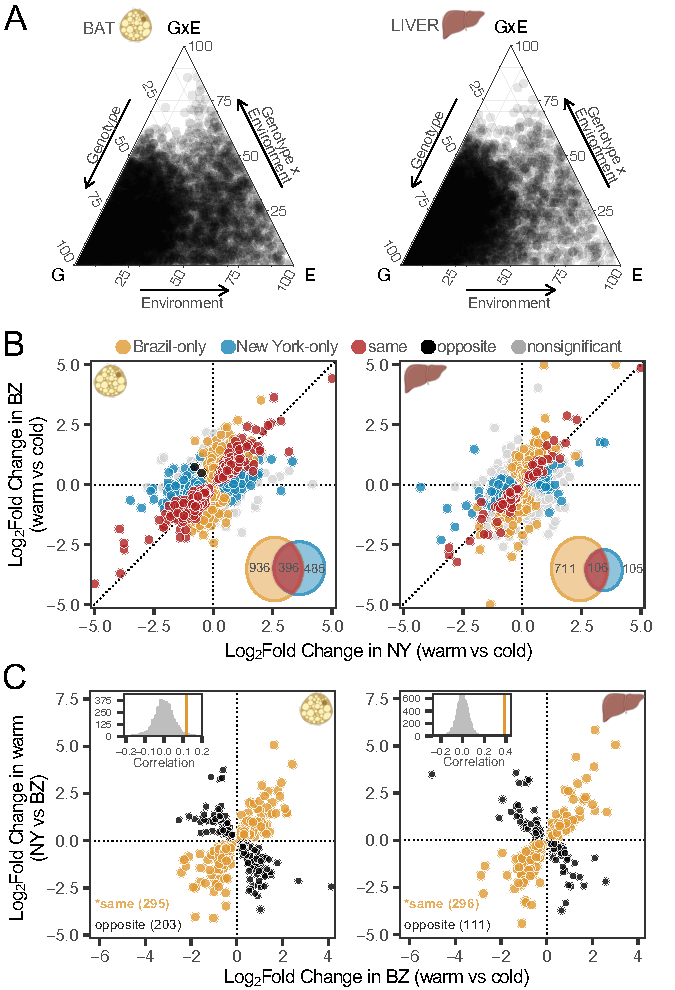
\includegraphics[width=1\columnwidth]{./figure_2.pdf}
  \caption{Gene expression patterns of New York and Brazil male house mice. Female-specific patterns are presented in Figure SX.}
\end{figure}

The strong patterns of divergence were also apparent when we categorized
differentially expressed genes as those showing genetic variation (G),
environmental variation {[}i.e., plasticity (E){]}, or genetic variation
for plasticity (i.e., G x E) (Figure 2B; Figure SX), genotype explained
the most variation, as the vast majority of differentially expressed
genes in both tissues exhibited strong patterns of divergence,
regardless of the environment (effect size of G
\textgreater\textgreater{} effect size of E; Fig 2B; Figure SX
(divergence expression)). (BUT) BAT showed greater proportion of E genes
compared to liver (diff effect sizes), highlighting the highly plastic
nature of BAT (fig Sx - BAT plasticity) and overlal tissue-specific
differences in gene expression plasticity.

Despite this strong signal of divergence, of genes (XXX) and (XXX)
showed genotype x environment interactions (GxE) in BAT and liver,
respectively (Figures 2C and SX(females)). (AND) Across both tissues,
Brazil mice harbored more DEG than New York mice (Figure 3), with New
York mice showing canalization of plasticity between environments
(Figure 2). - also include volcano plot of DEG for each tissue? (AND)
Given the large number of plastic genes in Brazil, we next asked whether
the plastic response of these genes correlated with expression
divergence between New York and Brazil lines. Specifically, we asked if
the logFC of Brazil warm and Brazil cold was positively correlated with
the logFC of New York warm and Brazil warm. (AND) Across both tissues,
plasticity in Brazil was positively correlated with divergence,
suggesting that overall patterns of expression plasticity in response to
cold temperatures are adaptive. consistent with previous studies in
house mice (Bittner et al.~2021). (THEREFORE) Together, these results
demonstrate that, while the majority of differentially expressed genes
show strong patterns of divergence (expression differences are
concordant across environments) across environments, a subset of genes
show genotype-specific regulation in response to temperature (i.e.,
genetic variation for plasticity (GxE)).

\hypertarget{genotype-by-sex}{%
\subsubsection{Genotype-by-Sex}\label{genotype-by-sex}}

Although males and females showed similar patterns of gene expression
across tissues and environments, we did identify genotype x sex
interactions for each tissue and environment separately (see Methods).
Specifically, males harbored more DEG than females and RESULTS Given the
strong influences of both tissue and sex (see Figure SX), we performed
downstream analyses for each tissue and sex separately. These results
again demonstrate that divergence is playing a significant role, while
tissue, sex, and environment specific effects play less roles.

\hypertarget{expression-divergence-is-predominantly-due-to-cis-regulatory-changes-which-are-robust-to-environmental-temperature}{%
\subsection*{\texorpdfstring{Expression divergence is predominantly due
to \emph{cis}-regulatory changes, which are robust to environmental
temperature}{Expression divergence is predominantly due to cis-regulatory changes, which are robust to environmental temperature}}\label{expression-divergence-is-predominantly-due-to-cis-regulatory-changes-which-are-robust-to-environmental-temperature}}
\addcontentsline{toc}{subsection}{Expression divergence is predominantly
due to \emph{cis}-regulatory changes, which are robust to environmental
temperature}

To investigate the gene regulatory mechanisms underlying expression
differences between New York and Brazil mice, we generated BAT and liver
RNA-seq from New York (dam) x Brazil (sire) F1 hybrids that were also
reared in warm or cold environments. Dominance of gene expression

Measuring gene expression in F1 hybrids allows us to discern if parental
gene expression differences are due to cis- and/or trans-acting changes
by assessing patterns of allele-specific expression (ASE): differences
in expression between alleles are indicative of cis-regulatory
divergence, while differences observed between parental lines but not in
F1 hybrids are due to trans-acting variation.

Overall, we detected a total of 5,898 genes with ASE based on the
presence of fixed differences between parental Brazil and New York lines
(see Methods), with both liver and BAT harboring similar numbers of gene
underlying regulatory divergence (Figure 4). These results demonstrate
that cis-regulatory evolution underlies divergence between wild mouse
populations, consistent with previous studies in house mice (refs).

Given that both New York and Brazil mice have adapted to divergent
thermal environments, we reasoned that temperature-dependent gene
regulation may play a role in local adaptation. We therefore asked how
the environment modulates gene regulatory evolution by comparing
patterns of cis- and trans-regulatory differences across environments.
Similar to differential expression patterns in the parents, the majority
of genes showed the same gene regulatory patterns between environments
(88\%), suggesting that cis- and trans-effects play larger roles in
expression divergence than that of plasticity. Moreover, when we
compared the difference in magnitude of cis- and trans-differences
between environments, we found that cis-regulatory changes were robust
to environmental temperature while trans-differences were greater
between environments for both tissues (Wilcoxon signed-rank test,
\emph{P} \textgreater{} 0.05; Figure 4B,4D - effect sizes). We also
found that the proportion of genes with only cis-divergence was the same
across environmental temperatures (Chi-square tests: BAT, p=0.51; liver
p=0.66), while the cold environment harbored a lower proportion of genes
with trans-divergence (Chi-square tests: BAT, p=0.0003; liver, p=0.02).
These results suggest that trans-effects are more sensitive to
environmental condition, consistent with previous studies (refs).

\begin{figure*}[t]
  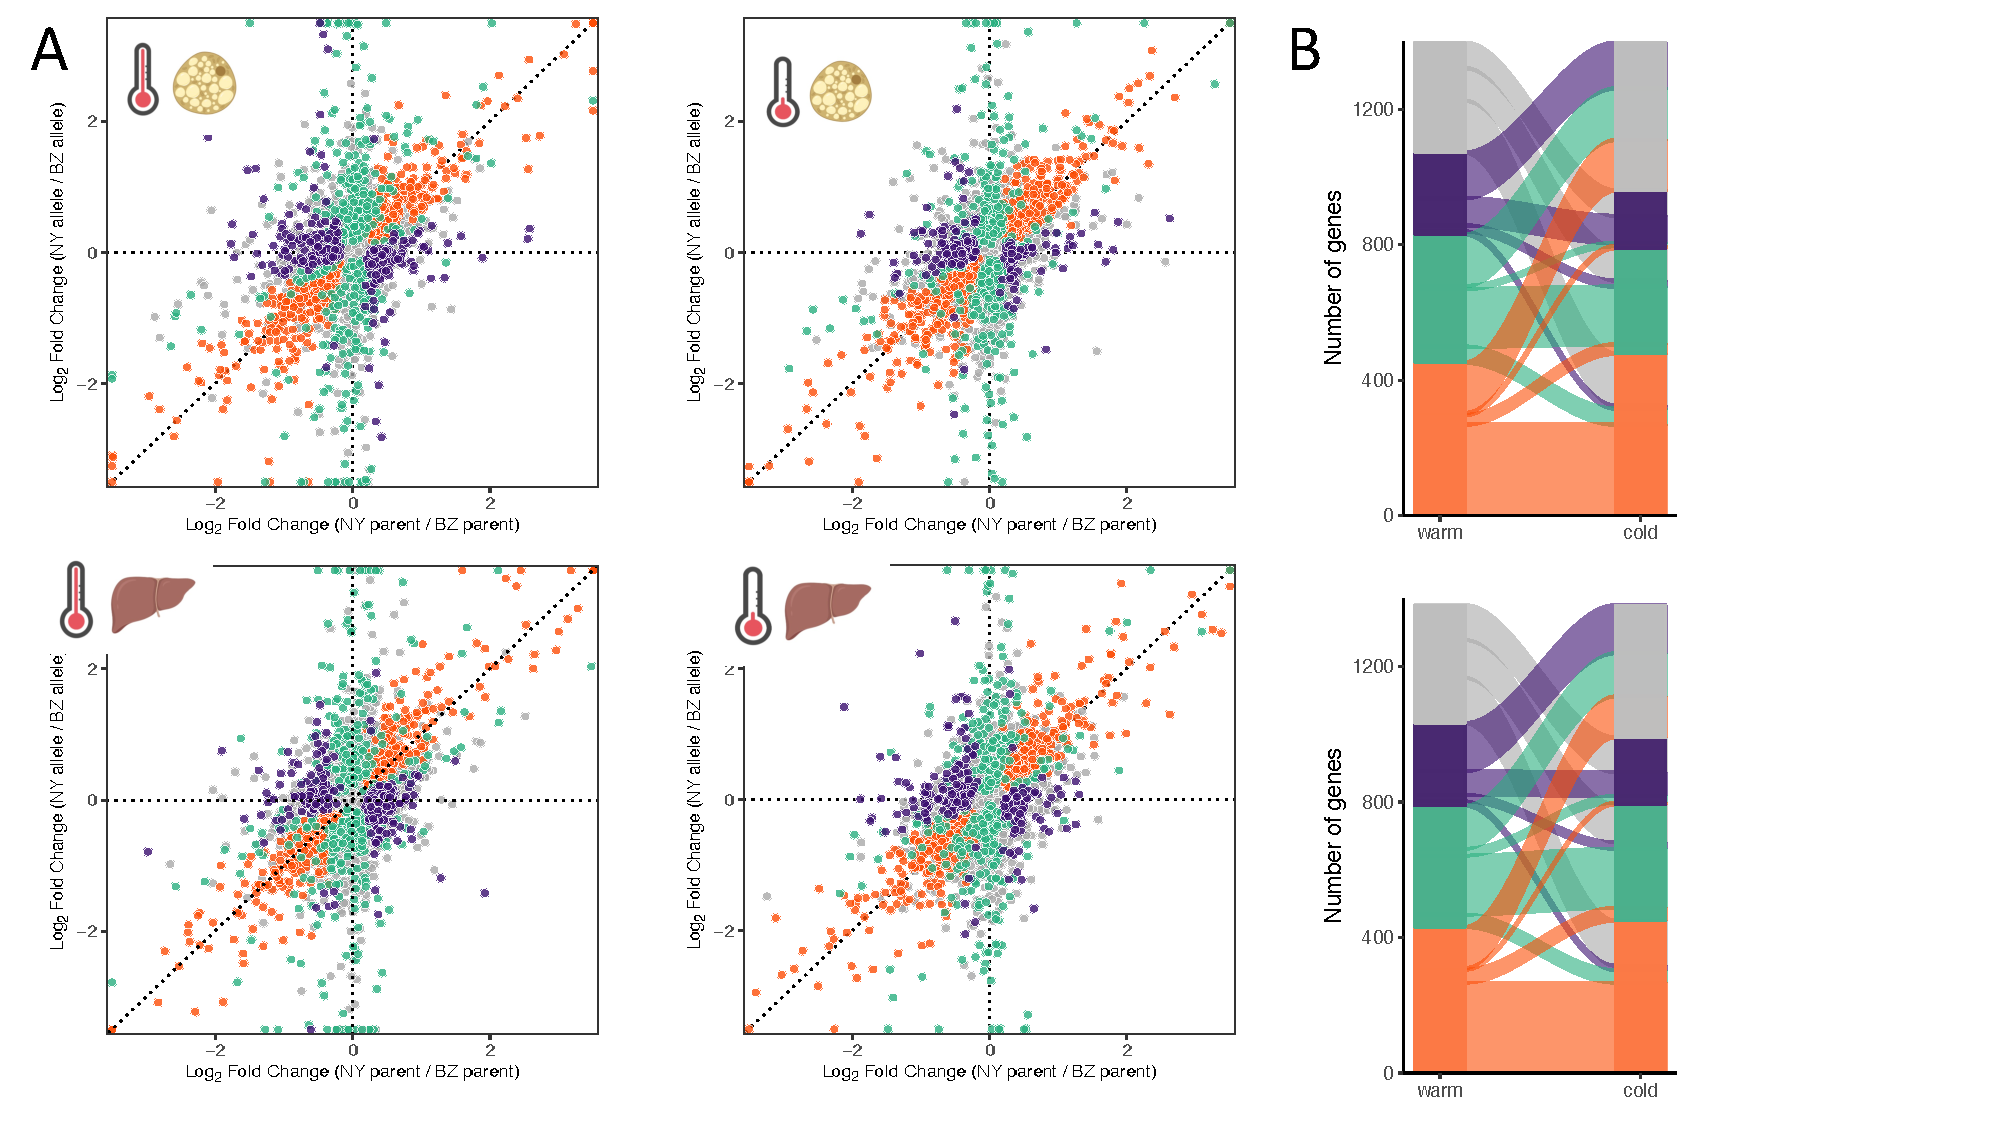
\includegraphics[width=\textwidth]{./figure_3.pdf}
  \caption{This is Figure 1, which introduces the awesome system of house mice we have. (A) Mice are found throughout North and South America, and throughout this invasive range, temperature is major climatic variable. We are using wild-derived inbred lines of house mice collected from upstate New York (brrrr) and equatorial Brazil (it's gettin' hot in here). (B) Mice collected from these localities show differences in thermoregulatory phenotypes after many generations in the lab, indicating a genetic basis. (C) For this study, specifically, we took an allele-specific approach across two tissues, two sexes, and two environments (2x2x2) to identify the gene regulatory signature of rapid adaptation.}
\end{figure*}

Although most gene regulatory patterns are robust to environment, genes
showing GxE patterns may be controlled by environment-specific
regulation. To robustly identify genes for which there was a significant
effect of temperature on regulatory divergence, we next asked if either
the \emph{cis} component and/or \emph{trans} component showed a
significant interaction with temperature.

\emph{Trans}-by-treatment identified for 19 genes in BAT and liver
(Table XX)(FDR\textless0.1). \emph{Cis}-by-treatment/temperature effects
were identified for 11 genes in BAT (gstt1, wars2, hsd11b1, itih5, dst,
tmed2, plbd1, cdh13, scd1, tmem45b, s100a13) and 4 in the liver (elovl3,
hmgcs2, wars2, ebpl) (FDR\textless0.1). Scd1 is a central lipogenic
enzyme catalyzing the synthesis of monounsaturated fatty acids and plays
an important role in basal and cold-induced thermogenesis. Scd1 is
required for maintaining body temperature under cold temperatures, and
mice from New York show higher average expression of this under warm
conditions in BAT than mice from Manaus. Elovl3 expression is also
involved in the response to exposure to cold stress and mutants show
defects in lipid recruitment in response to cold exposure. Where most of
these are cases where allele-specific expression differs in magnitude
between temperature treatments, we also observed cases where
allelic-specific expression was induced by one temperature treatment
(i.e., wars2, tmed2, cdh13, s100a13, ebpl, hmgcs2).

\hypertarget{cis-regulatory-changes-are-largely-tissue-biased-and-are-related-to-body-size-and-metabolism}{%
\subsection*{\texorpdfstring{\emph{Cis}-regulatory changes are largely
tissue-biased and are related to body size and
metabolism}{Cis-regulatory changes are largely tissue-biased and are related to body size and metabolism}}\label{cis-regulatory-changes-are-largely-tissue-biased-and-are-related-to-body-size-and-metabolism}}
\addcontentsline{toc}{subsection}{\emph{Cis}-regulatory changes are
largely tissue-biased and are related to body size and metabolism}

While both liver and BAT both play essential roles in homeostasis and
metabolism, these tissues have distinct functional properties that may
lend differentially to their role in environmental adaptation. Comparing
gene expression evolution in BAT and liver, we found regulatory
divergence to be largely tissue-biased. The majority of genes (80\%)
with evidence for regulatory divergence in at least one of the tissues
were not categorized as having the same underlying regulatory divergence
in the other tissue (2954/3672 genes). In particular, we found that
\emph{trans}- divergence was more likely to be restricted to one tissue
(with expression conserved between populations in the other), compared
to \emph{cis}- changes which were more often shared (\textgreater2-fold
more)(Chi-square test p\textless0.0001; Tables SX). This may reflect the
general observation of increased tissue-specificity of trans-effects
relative to cis-effects {[}15{]}.

Contrasting allele-specific expression measurements in BAT and liver for
paired hybrid samples, we identified 338 genes with evidence for
differential allele-specific expression between tissues (Figure 3A).
While the majority of these genes (77\%) showed significant
allele-specific expression in just one tissue, we also identified cases
where allele-specific was present in both tissues but with differences
in the magnitude or directionality (23\%). Forty-three genes of these
genes were found to have discordant allele-specific expression between
tissues, where the opposite parental allele was up-regulated between
tissues. Genes with tissue-biased ASE were enriched for metabolic
phenotypes (e.g., abnormal lipid homeostasis, q=0.00027; increased food
intake, q=0.036) and tissue specific functions and physiology (e.g.,
abnormal adipose tissue physiology, q=0.007; and abnormal liver
morphology (q=0.00097). \textless rerference petrov or pritchard, in
which they're excited about cis-genes that are found in one tissue
only\textgreater{}

Given that most regulatory divergence between New York and Brazil house
mice is governed in cis, and because cis-regulatory variations are often
drives of local adaptation (refs), we reasoned that genes with evidence
for allele-specific expression between lines should be enriched for
similar functional roles. In both the liver and BAT, genes with evidence
for cis- divergence were enriched for GO terms related to metabolic
processes, as well as the Reactome pathway for metabolism (Liver q=6.55
x10-8, BAT q=1.49 x 10-8) compared to the background set of genes that
were tested for allele-specific expression. Genes with cis- regulatory
changes in the liver were also enriched for several mutant phenotype
annotations for homeostasis and metabolism, including abnormal lipid
homeostasis (q= 6.248 x 10-5), abnormal cholesterol level (q=0.003), and
abnormal energy expenditure (q=0.001), abnormal triglyceride level
(q=0.008). Additionally, genes with cis- changes in the liver also
showed a greater than 2-fold enrichment of genes with mutant phenotypes
for abnormal susceptibility to weight gain (q=0.014), and were also
nominally significantly enriched for several other phenotypes related to
body weight, size, and composition (e.g., increased body size and
weight, increased food intake, abnormal percent body fat/body weight,
decreased susceptibility to diet-induced obesity) (Table SXX). Among
these are genes (i.e., bcat2, adam17) for which expression levels in the
liver and \emph{cis}-eQTL were previously associated with body mass
variation in wild populations of North American house mice {[}14{]} as
well as genes with well-documented roles in body weight variation other
species (e.g., lepr, fads2, bbs1, prkar2b). These results further
support the strong divergence in body size we see between NY and BZ
mice, as body size is canalized and shows no plasticity (Figure SX).

\hypertarget{selection-on-genes-with-cis-regulatory-divergence-in-wild-house-mouse-populations}{%
\subsection*{Selection on genes with cis-regulatory divergence in wild
house mouse
populations}\label{selection-on-genes-with-cis-regulatory-divergence-in-wild-house-mouse-populations}}
\addcontentsline{toc}{subsection}{Selection on genes with cis-regulatory
divergence in wild house mouse populations}

To understand regulatory divergence between these lines in the context
of genetic divergence between populations from these localities, we
analyzed population genomic data from wild-caught individuals. We
compared complete exomes sequenced at moderate coverage for 18
individuals captured in New Hampshire/Vermont (10
individuals)(NH/VT)(cite megan) and Manaus (8 individuals).

Genetic PCA clearly distinguished populations based on geography. Mice
from the Americas were compared to previously published population
genomic data from Eurasian populations of M. domesticus (cite
Harr)(Figure 4). LD-pruned genotype data clustered all individuals by
subspecies and M. m. domesticus by population-of-origin (Figure SX).
Consistent with the suggestion that mice from eastern North America are
most closely related to populations in northern Europe, mice from NH/VT
clustered most closely with mice from Germany (cite Tichy et al.~1994,
Morgan et al.~BioRxiv paper).

To identify genetic signatures of adaptation in house mice from the
Americas, we performed a scan for regions of genetic differentiation
consistent with selection using a normalized version of the population
branch statistic (PBSn1). PBSn1 captures loci where allele frequencies
are especially differentiated in a focal population when compared with
two other populations (Yi et al.~2010; Crawford et al.~2017). We used
this test to identify highly differentiated loci in our focal
populations in the Americas, Manaus and New York, relative to Eurasian
populations (see Methods). In total, 83,538 and 84,420 non-overlapping
five-SNP windows were analyzed for Manaus and NH/VT, respectively. We
considered windows as outliers if they fell within the top 1\% of
windows for PBSn1 score. Outlier windows in NH/VT and Manaus overlapped
538 and 530 genes, respectively (File SX).

\textless Justification for looking at cis- overlap.\textgreater{} Next,
we overlapped candidate regions for selection based on PBSn1 outlier
windows with genes for which we identified evidence for cis- regulatory
changes in BAT or the liver. In NH/VT, we identified 99 outlier windows
that overlapped 64 genes with evidence for cis- regulatory divergence
(Figure 4). These genes were enriched for mutant phenotypes related body
size and growth relative to other genes with cis- divergence between
populations: (1) growth/size/body region phenotype (q=0.008; 1.74-fold
enrichment, 30 genes), (2) abnormal postnatal growth/weight/body size
(q=0.026; 1.97-fold enrichment, 23 genes), and (3) abnormal body
composition (q=0.05; 2-fold enrichment, 18 genes). This set included
genes whose expression in the liver was previously associated with body
mass variation in natural populations of North American house mice
(bcat2, col6a1, col5a2, col3a1). Additionally, this set included genes
implicated in obesity and metabolic phenotypes in humans (e.g., wrn,
plaat3, prkar2b, sulf2, smoc1) . In Manaus, we identified an overlap of
68 outlier windows overlapping 37 genes with evidence for cis-
regulatory divergence (Figure SX). These genes were enriched for
homeostasis/metabolism phenotypes (q=0.04, 1.62-fold enrichment, 20
genes) and as well as several non-metabolic phenotypes (e.g., integument
phenotype, abnormal locomotor activation) relative to a background of
genes with evidence for cis- divergence.

For the NH/VT comparison, we found that the overlap between genes with
cis- regulatory divergence and outlier windows was greater than expected
by chance (hypergeometric test, p=0.0017, 1.45-fold enrichment), where
we do not observe this enrichment for Manaus (p=0.16). Additionally,
genes with evidence for cis- regulatory divergence showed higher average
PBSn1 than other genes when NH/VT is a focal population (Permutation
test, p\textless0.00005), but not when Manaus was a focal population
(p=0.91).

\hypertarget{discussion}{%
\section*{Discussion}\label{discussion}}
\addcontentsline{toc}{section}{Discussion}

Understanding how both genetic and environmental variation influence
gene regulation is essential to understanding adaptive evolution. Here,
we utilized allele-specific expression to characterize cis and trans
changes underlying divergence and plasticity in temperate and tropical
house mice. We found that the majority of gene expression differences
showed concordant patterns of regulatory divergence across environments,
suggesting that genetic effects are more pervasive than environmental
effects. In particular, we found that most regulatory divergence was
underlined by cis-regulatory variation, and that these cis-effects were
highly independent of temperature. These results are consistent with
previous studies in yeast (Smith and Kruglyak 2008; Tirosh et al.~2009;
Naranjo et al.~2015); (Li et al.~2006); (Chen et al.~2015); (Cubillos et
al.~2014) in which most concordant expression differences across
environments are controlled by conserved cis effects. Moreover, the
universal patterns in the stability of cis-regulatory variation further
illustrates the significance of cis-acting factors in adaptive evolution
(Wittkopp et al.~2008; Emerson et al.~2010; Massouras et al.~2012; Tung
et al.~2015; Verta and Jones 2019). Overall, our results demonstrate
that cis-regulatory variation plays a significant role in the divergence
of North and South American house mice.

\hypertarget{rapid-divergence-of-introduced-populations-of-house-mice}{%
\subsection{Rapid divergence of introduced populations of house
mice}\label{rapid-divergence-of-introduced-populations-of-house-mice}}

These results highlight that divergence is a major axis of expression
variation in house mice. Divergence between subspecies (Mack et
al.~2016) resulted in about 9K fixed SNPS. Here, almost 6K fixed SNPs.

Changes in the environment preferentially impacted trans-regulation
profiles in house mice compared to cis-regulation (Tables 1 and 2;
Figure 2), suggesting that trans-effects play a more pronounced role in
gene expression plasticity. Greater sensitivity of trans-effects to the
environment is in strong agreement with previous studies in yeast (Smith
and Kruglyak 2008; Tirosh et al.~2009; Naranjo et al.~2015), nematodes
(Li et al.~2006), flies (Chen et al.~2015), and plants (Cubillos et
al.~2014). The generality of trans-effects being more sensitive across
environmental conditions may be due to the role trans-acting factors
play in signaling pathways that become activated in response to
environmental change (Ehrenreich and Pfennig 2016). Moreovoer, the large
mutational target space of trans-regulatory variants make them much more
pleiotropic than cis effects (Denver et al.~2005; Landry et al.~2007),
allowing them to impact the regulation of many genes that are contingent
upon an environmental stimulus (Promislow 2005). Indeed, we found that
the effect sizes of trans were greater than that of cis across both
tissues in house mice (Figure S4), suggesting that much of expression
plasticity we observed is governed by changes in trans.

Gene regulation is not only dependent on environmental conditions but it
is also tissue specific (GTEx). Although both liver and BAT exhibited
similar levels of cis- and trans-regulatory variation across
enviornments (Table 1), we did observe more cis- and
trans-by-temperature effects in BAT compared to liver (Table S1). These
patterns may reflect the developmentally plastic nature of BAT in
response to cold temperatures (Cannon and Nedergaard 2004).
Alternatively, these patterns may reflect differences in pleiotropy or
tissue-specificity. For example, threespine sticklebacks show a
preponderance of both cis (Verta and Jones 2019) and trans (Hart et
al.~2018) regulation underlying parallel environmental adaptation. The
discrepancies between the two studies are likely a result of differences
in tissues analyzed, as the genetic architectures of simple and complex
tissues differ from the effect of heterogeneity (Hart et al.~2018; Verta
and Jones 2019). Similar influences may be contributing to differences
seen between BAT and liver. For example, BAT is a more heterogeneous
tissue than the liver, with varying levels of lipid droplets and
mitochondria (Ikeda et al.~2018; Oguri and Kajimura 2020). Moreover, the
greater proportion of trans-by-temperature effects in BAT compared to
the liver may be indicative of BAT being more specialized and
pleiotropic, especially in terms of plasticity. Overall, these results
highlight the importance of investigating the effects of gene regulation
across multiple tissues.

Finally, the role of expression plasticity in facilitating or
constraining adaptation has received considerable attention in the last
few years (Ghalambor et al.~2015; Velotta et al.~2018; Campbell-Staton
et al.~2021; Josephs et al.~2021). Although numerous studies have
identified roles for both adaptive and non-adaptive expression
plasticity, very few studies have characterized the underlying
regulatory architecture of such patterns (He et al.~2021). We overlapped
cis- and trans-by-temperature candidates with patterns of adaptive
plasticity previously identified (Ballinger and Nachman, in prep) and
found that genes exhibiting adaptive plasticity are underlined by both
cis-by-treatment and trans-by-treatment effects (Figure 3).
Interestingly, most genes exhibiting adaptive plasticity are
constitutively expressed across warm and cold environments in New York
mice. Although we do not have direct evidence for genetic assimilation
(Waddington 1952, 1953; Crispo 2007), these candidates illustrate the
potential regulatory mechanisms underlying genetic assimilation. For
example, cis regulatory variants could rapidly canalize expression
through the loss or gain of specific binding sites for conditionally
expressed transcription factors, thereby decoupling a gene's expression
from the environment (Ehrenreich and Pfennig 2016). Alternatively, trans
effects could activate environmentally-sensitive signaling pathways in
the absence of an environmental cue, causing a gene's expression to be
constitutively expressed (Yvert et al.~2003; Ehrenreich and Pfennig
2016). However, these hypotheses do not consider the effects of gene
regulatory networks nor identify causal mutations of candidate genes.
Thus, future work is needed to identify causal mutations underlying
adaptive plasticity and genetic assimilation (Corl et al.~2018; van der
Burg et al.~2020). Regardless, these are exciting candidates for further
investigation into the molecular and regulatory underpinnings of
adaptive plasticity in house mice.

\hypertarget{methods}{%
\section*{Methods}\label{methods}}
\addcontentsline{toc}{section}{Methods}

\hypertarget{mice}{%
\subsubsection*{Animals and experimental design}\label{mice}}
\addcontentsline{toc}{subsubsection}{Animals and experimental design}

We used two wild-derived inbred lines of house mice collected from
upstate New York (SARA) and equatorial Brazil (MANA). The establishment
of these lines and the experimental design implemented in this study
have been described previously (Ballinger and Nachman, 2022). Briefly,
we generated F1 hybrids by crossing a New York female with a Brazil
male. All experimental animals were born at room temperature (20oC). We
weaned and singly housed SARA, MANA, and F1 hybrids at \textasciitilde3
weeks of age. We split 3.5-week-old full-sibs and F1 hybrids into
size-matched experimental groups across cold (5oC) and warm (21oC)
treatments. Mice were kept in their respective experimental environment
up until \textasciitilde12 weeks of age, at which point individuals were
euthanized via cervical dislocation. We took standard museum
measurements and then rapidly dissected and preserved liver and brown
adipose tissue in RNAlater at 4oC overnight and moved to -80oC until RNA
extraction. Skins were removed and dried for subsequent thermal
conductance measruements (ref; see SI methods). All experimental
procedures were in accordance with the UC Berkeley Institutional Animal
Care and Use Committee (AUP-2017-08-10248). Food and water were provided
\emph{ad libitum}.

\hypertarget{rna-extraction-library-preparation-and-sequencing}{%
\subsubsection*{RNA extraction, library preparation, and
sequencing}\label{rna-extraction-library-preparation-and-sequencing}}
\addcontentsline{toc}{subsubsection}{RNA extraction, library
preparation, and sequencing}

We extracted total RNA from both liver and BAT from each sample (n =
\textasciitilde6 per genotype/sex/treatment/tissue) using the RNeasy
PowerLyzer Kit (QIAGEN). We generated Illumina cDNA libraries from 1 ug
of purified RNA using KAPA Stranded mRNA-Seq Kit (Illumina), and
uniquely indexed libraries using unique dual indexes (Illumina).
Libraries were pooled in equal molar concentration and sequenced on one
lane each of 150 bp paired-end NovaSeq S1 and NovaSeq S4 at the Vincent
J. Coates Genomics Sequencing Center at UC Berkeley. We filtered raw
reads below a Phred quality score of 15 and trimmed adapter sequences
using fastp (Chen et al.~2018).

\hypertarget{parental-gene-expression-analyses}{%
\subsubsection*{Parental gene expression
analyses}\label{parental-gene-expression-analyses}}
\addcontentsline{toc}{subsubsection}{Parental gene expression analyses}

After cleaning and trimming parental sequences of MANA and SARA, we
mapped reads to the Mus musculus reference genome (GRCm38/mm10) using
STAR (Dobin et al.~2013). We counted reads overlapping exons using HTSeq
(Anders et al.~2015) based on the Ensembl GRCm38.98 annotation. After
pre-processing and filtering, we retained \textgreater14K genes for
downstream analyses. We detected \textasciitilde14K expressed genes that
were shared across all samples (XXX for warm-reared mice, XXX for
cold-reared mice; normalized counts -- 10 reads per gene across all
samples in each tissue separately). We imported raw count data into R
(v.4.1) and used DESeq2 (Love et al.~2014) to quantify expression
patterns by fitting a generalized linear model following a negative
binomial distribution. First, we determined effects of genotype,
environment, and genotype-by-environment on expression patterns between
lines for each tissue separately. We then computed differential
expression between lines with the model population + environment +
population*environment. We removed genes with a mean fewer than 10 reads
across samples per tissue. Lastly, we used a Benjamini-Hochberg multiple
test correction (Benjamini and Hochberg 1995) on the resulting P-values
and considered genes with a false discovery rate (FDR) smaller than 0.05
to be significantly differentially expressed.

\hypertarget{identifying-variants-between-parental-lines}{%
\subsubsection*{Identifying variants between parental
lines}\label{identifying-variants-between-parental-lines}}
\addcontentsline{toc}{subsubsection}{Identifying variants between
parental lines}

To identify differences between lines for allele-specific read
assignment, SNP calling was performed on whole genome sequence data from
one female each of MANA and SARA. Genomic reads were mapped with Bowtie2
(Langmead and Salzberg 2012) to the mm10 reference genome (setting:
--very-sensitive) obtained from Ensembl. Duplicates were marked with the
Picard tool MarkDuplicates and then the GATK tools HaplotypeCaller and
GenotypeGVCFs were used for joint genotyping across genomic samples. We
filtered for low quality SNP calls with VariantFiltration (QD
\textless{} 2.0; QUAL \textless{} 30.0; FS \textgreater{} 200;
ReadPosRankSum \textless{} -20.0). To reduce the influence of genotyping
error on allele-specific expression, we mapped RNAseq reads from all
individuals and then counted allele-specific reads aligned to each site
we genotyped with the GATK tool ASEReadCounter. Sites for which we did
not have coverage of at least 5 reads from each population-specific
allele were excluded. These SNPs were then used for identifying
allele-specific reads.

\hypertarget{mapping-allele-specific-reads}{%
\subsubsection*{Mapping allele-specific
reads}\label{mapping-allele-specific-reads}}
\addcontentsline{toc}{subsubsection}{Mapping allele-specific reads}

For allele-specific expression analyses, reads from hybrid individuals
were mapped to the mouse reference genome (GRCm38/mm10) using STAR. We
used WASP (van de Geijn et al.~2015) to reduce the potential for
reference mapping bias. Reads that overlapped a population-specific
variant and that passed WASP filtering were retained for our
allele-specific expression analysis. Reads overlapping informative
variants were separated into allele-specific pools (NY, BR) based on
genotype for quantification. We used HTSeq to count the number of reads
associated with each gene per population based on the overlap of reads
and annotated exonic regions based on the Ensembl GRCm38.98 annotation.
We examined per site allelic reads with ASEReadCounter to quantify read
mapping bias. Proportions of reads overlapping the references
vs.~alternative allele (REF allele / (ALT allele + REF allele)) show a
median 0.5 across samples (Figure S5). Consequently, we do not find
evidence for reference mapping bias. Overall, a total of 5,861 genes
were tested for allele-specific expression based on the presence of
fixed differences between Brazil (MANA) and New York (SARA) lines.

\hypertarget{identifying-cis-and-trans-divergene}{%
\subsubsection*{Identifying cis- and trans-
divergence}\label{identifying-cis-and-trans-divergene}}
\addcontentsline{toc}{subsubsection}{Identifying cis- and trans-
divergence}

To characterize regulatory divergence in warm and cold temperature
treatments, we compared expression in Brazil and New York lines (F0
generation) with differences in expression in alleles in a hybrid (F1
generation). Differential expression between alleles in hybrids is
evidence for cis- regulatory divergence, where differences in the ratio
of expression between alleles in a hybrid and between genes in the F0
generation are evidence for trans divergence. Differential expression in
the F0 generation (parents) was inferred by analyzing raw counts using
the DESeq2 package (see above). To identify genes with evidence of
allelic imbalance in hybrid individuals, we took reads that mapped
preferentially to either New York or Brazil alleles and fit these to a
model with allele (NY vs.~BZ), sample (individual), and tissue (BAT,
liver) for hybrid male samples (\textasciitilde temperature +
individual:temperature + allele:temperature) in DESeq2. The trans
component was assessed through a Fisher's Exact Test on reads mapping to
each parental allele in the hybrid versus parental read counts, summed
over all replicates. We randomly down-sampled to account for library
size differences between parental and F1 replicates. P-values for each
test were corrected for false-discovery rate with the Benjamini-Hochberg
method. Tests with FDR \textless{} 0.05 were considered significant.
Genes with differences in expression between alleles in the hybrid and
expression in the F0 generation and without a difference between these
ratios (via the Fisher's Exact Test) were considered divergent in cis
alone. Genes without allele-specific expression in hybrids but
differential expression in the F0 generation and a significant
difference in these ratios were considered divergent in trans alone.
Cases where we identified a significant trans component and divergence
in either alleles in the hybrid or expression in the F0 generation were
indicative of cis and trans divergence together.

\hypertarget{population-genomic-analyses}{%
\subsubsection*{Population genomic
analyses}\label{population-genomic-analyses}}
\addcontentsline{toc}{subsubsection}{Population genomic analyses}

\hypertarget{data-availability-data-availability-.unnumbered}{%
\subsubsection{Data availability (\#data-availability
.unnumbered)}\label{data-availability-data-availability-.unnumbered}}

\hypertarget{supporting-information-si}{%
\subsection*{Supporting Information
(SI)}\label{supporting-information-si}}
\addcontentsline{toc}{subsection}{Supporting Information (SI)}

Authors are limited to no more than 10 SI files, not including movie
files. Authors who place detailed materials and methods in SI must
provide sufficient detail in the main text methods to enable a reader to
follow the logic of the procedures and results and also must reference
the online methods.

\hypertarget{si-text}{%
\subsubsection*{SI Text}\label{si-text}}
\addcontentsline{toc}{subsubsection}{SI Text}

Supply Word, RTF, or LaTeX files (LaTeX files must be accompanied by a
PDF with the same file name for visual reference).

\hypertarget{si-figures}{%
\subsubsection*{SI Figures}\label{si-figures}}
\addcontentsline{toc}{subsubsection}{SI Figures}

Provide a brief legend for each supporting figure after the supporting
text. Provide figure images in TIFF, EPS, high-resolution PDF, JPEG, or
GIF format; figures may not be embedded in manuscript text. When saving
TIFF files, use only LZW compression; do not use JPEG compression. Do
not save figure numbers, legends, or author names as part of the image.
Composite figures must be pre-assembled.

\hypertarget{si-tables}{%
\subsubsection*{SI Tables}\label{si-tables}}
\addcontentsline{toc}{subsubsection}{SI Tables}

Supply Word, RTF, or LaTeX files (LaTeX files must be accompanied by a
PDF with the same file name for visual reference); include only one
table per file. Do not use tabs or spaces to separate columns in Word
tables.

\hypertarget{si-datasets}{%
\subsubsection*{SI Datasets}\label{si-datasets}}
\addcontentsline{toc}{subsubsection}{SI Datasets}

Supply Excel (.xls), RTF, or PDF files. This file type will be published
in raw format and will not be edited or composed.

\showmatmethods
\showacknow
\pnasbreak

\hypertarget{refs}{%
\section*{refs}\label{refs}}
\addcontentsline{toc}{section}{refs}



% Bibliography
% \bibliography{pnas-sample}

\end{document}
